\documentclass[border=4pt]{standalone}

\usepackage[T1]{fontenc}
\usepackage[utf8]{inputenc}
\usepackage{amsmath}
\usepackage{xcolor}
\usepackage{tikz}
\usetikzlibrary{positioning, calc, arrows.meta, backgrounds}

\definecolor{keepc}{RGB}{76,160,90}     % kept advantages : green
\definecolor{zeroc}{RGB}{205,90,75}      % zeroed (biased) : red
\definecolor{valc}{RGB}{70,130,200}      % value targets : blue

\begin{document}

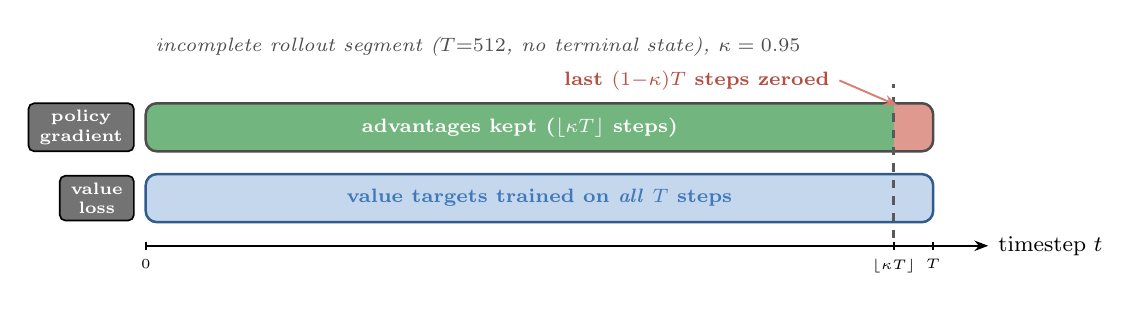
\begin{tikzpicture}[font=\small, >={Stealth[length=5pt]},
  % black "pill" row labels (signature element) ──
  rowpill/.style={fill=black!55, draw=black, line width=0.6pt, text=white, rounded corners=2pt,
                  align=center, inner xsep=4pt, inner ysep=2.5pt, font=\fontsize{6pt}{7pt}\selectfont\bfseries},
]

% rollout segment: t = 0..T=512  ->  plot x = 0..10 ; kT = 0.95*T -> x = 9.5

%% ── header ───────────────────────────────────────────────────────
\node[anchor=west, font=\scriptsize\itshape, text=black!70] at (0,2.95)
  {incomplete rollout segment ($T{=}512$, no terminal state), $\kappa = 0.95$};

%% ── policy-gradient bar (advantages) : rounded, two-tone, strong border ──
\begin{scope}
  \clip[rounded corners=4pt] (0,1.62) rectangle (10,2.23);
  \fill[keepc!78] (0,1.62) rectangle (9.5,2.23);
  \fill[zeroc!62] (9.5,1.62) rectangle (10,2.23);
\end{scope}
\draw[rounded corners=4pt, black!70, line width=0.9pt] (0,1.62) rectangle (10,2.23);
\node[font=\scriptsize\bfseries, white] at (4.75,1.925) {advantages kept ($\lfloor\kappa T\rfloor$ steps)};
\node[rowpill, left=4pt of {(0,1.925)}] {policy\\gradient};

%% ── value bar (returns) : rounded, strong border ────────────────
\begin{scope}
  \clip[rounded corners=4pt] (0,0.72) rectangle (10,1.33);
  \fill[valc!32] (0,0.72) rectangle (10,1.33);
\end{scope}
\draw[rounded corners=4pt, valc!70!black, line width=0.9pt] (0,0.72) rectangle (10,1.33);
\node[font=\scriptsize\bfseries, text=valc!92!black] at (5,1.025) {value targets trained on \emph{all} $T$ steps};
\node[rowpill, left=4pt of {(0,1.025)}] {value\\loss};

%% ── boundary ─────────────────────────────────────────────────────
\draw[dashed, black!65, line width=1pt] (9.5,0.52) -- (9.5,2.48);

%% ── callout on the zeroed tail (lowered, clear of the header) ───
\node[font=\scriptsize\bfseries, text=zeroc!88!black, align=center] (cz) at (7.0,2.52)
  {last $(1{-}\kappa)T$ steps zeroed};
\draw[->, zeroc!78, line width=0.7pt] (cz.east) -- (9.55,2.20);

%% ── timeline axis ───────────────────────────────────────────────
\draw[->, line width=0.7pt] (0,0.42) -- (10.7,0.42) node[right, font=\footnotesize] {timestep $t$};
\foreach \x/\lab in {0/{$0$}, 9.5/{$\lfloor\kappa T\rfloor$}, 10/{$T$}}{
  \draw[line width=0.6pt] (\x,0.37) -- (\x,0.47);
  \node[below, font=\tiny] at (\x,0.37) {\lab};
}

\end{tikzpicture}

\end{document}
